\section{Laboratory work implementation}

\subsection{Tasks and Points}

Aici trebuie sa fie lista de task-uri care au fost implementate.

\end{enumerate}

\subsection{Analiza lucrarii de laborator}

Adauga link la repozitoriul tau.
Explica fiecare din task-urile realizate. Explica acesta cu cuvintele tale. Cu cit mai bine va fi explicat,
cu atit mai putine intrebari vei avea la aparare. Pentru a adauga referintele si completarea bibliografie se foloseste instructiunea \ref{referinta}. Referinta se va completa in fisirulul 

\subsection{Imagini}

Adauga cite cel putin o imagine (sau mai multe) pentru fiecare functionalitate adaugata.

% Exemplu de figura cu titlu, si referinta, label

\begin{figure}[!ht]
\centering
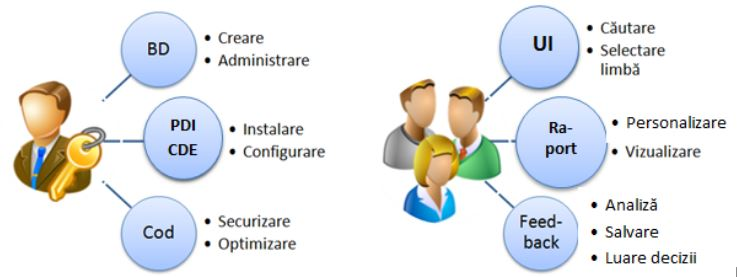
\includegraphics[width=1.0\textwidth]{schema}
\caption{Titlul imaginii, \cite{ImRef}}
\label{Im_label}
\end{figure}

% Exemplu de listing. Cum sa adaugi cod sursa in functie de limbajul de programare

\lstinputlisting[style=mystyle, language=SQL, caption={Titlul listing-ului}, label=paymentview,]{sourcecode/minmax.sql}


% Exemplu de tabel. El poate fi efectuat si exportat in forma online: 
% http://www.tablesgenerator.com/

\begin{table}[!ht]
\centering
\caption{Cerințele hardware pentru instrumentul Pentaho}
\label{hardware}
\begin{tabular}{|l|l|}
\hline
RAM      & Cel puțin 2GB             \\ \hline
HDD      & Cel puțin 1GB             \\ \hline
Procesor & Dual-core AMD64 sau EM64T \\ \hline
\end{tabular}
\end{table}




\clearpage